
\documentclass[12pt, titlepage]{scrartcl}
\setkomafont{disposition}{\normalfont\bfseries}

\title{\textbf{\textit{Astrea}} Constellation }
\subtitle{Project Charter \vspace{7cm}}


%\author{ Pol Fontanes Molina, \and  Victor Martinez Viol, \and David Morata Carranza,
%        Josep Maria Serra Moncunill, \and
%        Eva Mar\'{i}a Urbano Gonz\'{a}lez,  \and
%        Nando Herr\'{a}n Albelda, \and
%        Lluís Foreman Campins, \and
%        Oscar Fuentes Mu\~noz, \and
%        Silvia Gonz\'{a}lez Garc\'{i}a, \and
%        Laura Pla Olea, \and
%        Joan Cebrian,  \and
%        Josep Puig Ruiz, \and
%        Roger Fraixedas	, \and
%        Marina Pons, \and
%		Sergi Tarroc, \and
%		Xavi Ti\'{o}, \and
%		Boyan Naydenov
%}
\author{\emph{Group 4}}

\date{\textit{\today}}

\usepackage{blindtext}
\usepackage[utf8]{inputenc}
\usepackage{fancyhdr}
\usepackage{lastpage}
\usepackage{booktabs}
\usepackage{pdfpages}
\pagestyle{fancy}

\lhead{\textit{Astrea}}
\chead{}
\rhead{ESEIAAT
Engineering Projects Department}
\lfoot{}
\cfoot{ \thepage \hspace{1pt}/\pageref{LastPage}}
\rfoot{}


\begin{document}
\maketitle
\tableofcontents
\pagebreak
\pagebreak


\section{Aim of the project}
Design of a \textbf{satellite constellation} dedicated to  communications relay between LEO Cubesats. 


\section{Scope of the project}
A project of such magnitude comprises a large number of tasks, nevertheless, some of them are beyond the scope of this project. The ones that are actually on its scope are:

\begin{itemize}
  \item \textit{Design of the orbits}
  \item \textit{Design of the Cubesats}
  \item \textit{Lunch system}
  \item \textit{Lunching procedure}
  \item \textit{Design of the ground station}
  \item \textit{Communication protocols}
  \item \textit{End of life procedure}
\end{itemize}

\section{Basic requirements of the project}
\begin{table}[htb]
\centering
\caption{Project Requirements}
\label{my-label}
\begin{tabular}{@{}ll@{}}
\toprule
\textbf{Feature} & \textbf{Description}                                                                                                                                                          \\ \midrule
1                & \begin{tabular}[c]{@{}l@{}}Provide \textbf{low latency} communication relay between LEO nanosatellites \\ and the ground.\end{tabular}\vspace{0.3cm}                                                 \\
2                & \begin{tabular}[c]{@{}l@{}}Back-up systems in case some satellite subsystems fails. Therefore,\\ \textbf{guarantee }the service.\end{tabular}\vspace{0.3cm}                                                                                        \\
3                & \begin{tabular}[c]{@{}l@{}}Use modern and more efficient solutions in order to \textbf{reduce} mass, \\ volume and other critical parameters. Examples are SDR, DTN, etc.\end{tabular}\vspace{0.3cm}                                                 \\
4                & \begin{tabular}[c]{@{}l@{}}Combine satellite nodes with some ground nodes in order to improve\\ reliability.\end{tabular}\vspace{0.3cm}                                                                                                     \\ \bottomrule
\end{tabular}
\end{table}

\section{Justification } \label{justification}
\paragraph{}Nowadays, different universities, research centers and an incresing amount of companies are developing small satellites more and more. These are much more economic and therefore, today’s space access achievability has increased substantially. With that, small satellite constellation missions have been proposed, such as \textbf{QB50} project.

\paragraph{}These complex systems already need to configure and maintain dynamic routes, manage intermediate nodes, and reconfigure themselves to achieve mission objectives. Hence, inter-satellite is both important for satellites that fly in formation and need interconnection, and for single nanosatellites that may require low-latency communication with the ground.


\section{Organization of the group}


\subsection{Hierarchy}
\paragraph{}
Designing a nanosatellite constellation is quite ambitious and requires lots of work because there are many things to consider. In order to build a work strategy, the project is divided in tasks that will be described later on. As the different tasks depend on each other, the project members have decided to follow a hierarchy. Every task is developed by a small team between 2 and 5 people depending on the amount of work the task requires.
\paragraph{}
Each small team has to have a coordinator which has two principal functions. The first one is to manage the group so he is responsible for the good organisation and progression of the task. The second is that he is the voice of the team. That means that the coordinator is the one who represents his work team when transferring information to the other group coordinators and the project managers and vice versa. 
\paragraph{}
Finally over all the teams there is the project manager who maintains order, ensures the project progress and manages people for major decisions. Finally there is also a secretary in charge to write the minutes of each meeting.


\subsection{Documents Organisation}
\paragraph{}
Nowadays, the internet is crucial for teamwork because it provides lots of tools that improve networking such as sharing documents, communicating and even collaborating working. The Astrea team has 17 members so it is essential to define protocol to organise all the documents and information found to take advantage of resources. 
\paragraph{}
The principal communication tool used is \textit{Slack} which is a platform specialised in team communication. \textit{Slack} defines itself as a real-time messaging, achieving and search for modern team which is interesting for us because it allows the group to communicate at all times for punctual doubts and small decisions. For major decisions a date is specified by a \textit{doodle} to meet.
\paragraph{}
Moreover, to share documents we use two platforms: \textit{Slack} and \textit{BSCW}. On \textit{Slack} we put first drafts or documents that can be interesting. \textit{BSCW} is the main information storage because information and documents are stocked and organised in folders.
\paragraph{}
At last, the text editor used to develop the project is Latex which combined with Git allows us to work remotely on a same document without overriding someone else's work. This work system is really interesting for such a big group in order to work on the same document while keeping a record of the changes. 

\section{Planning of the project}

\subsection{Tasks identification from work breakdown structure (WBS)}
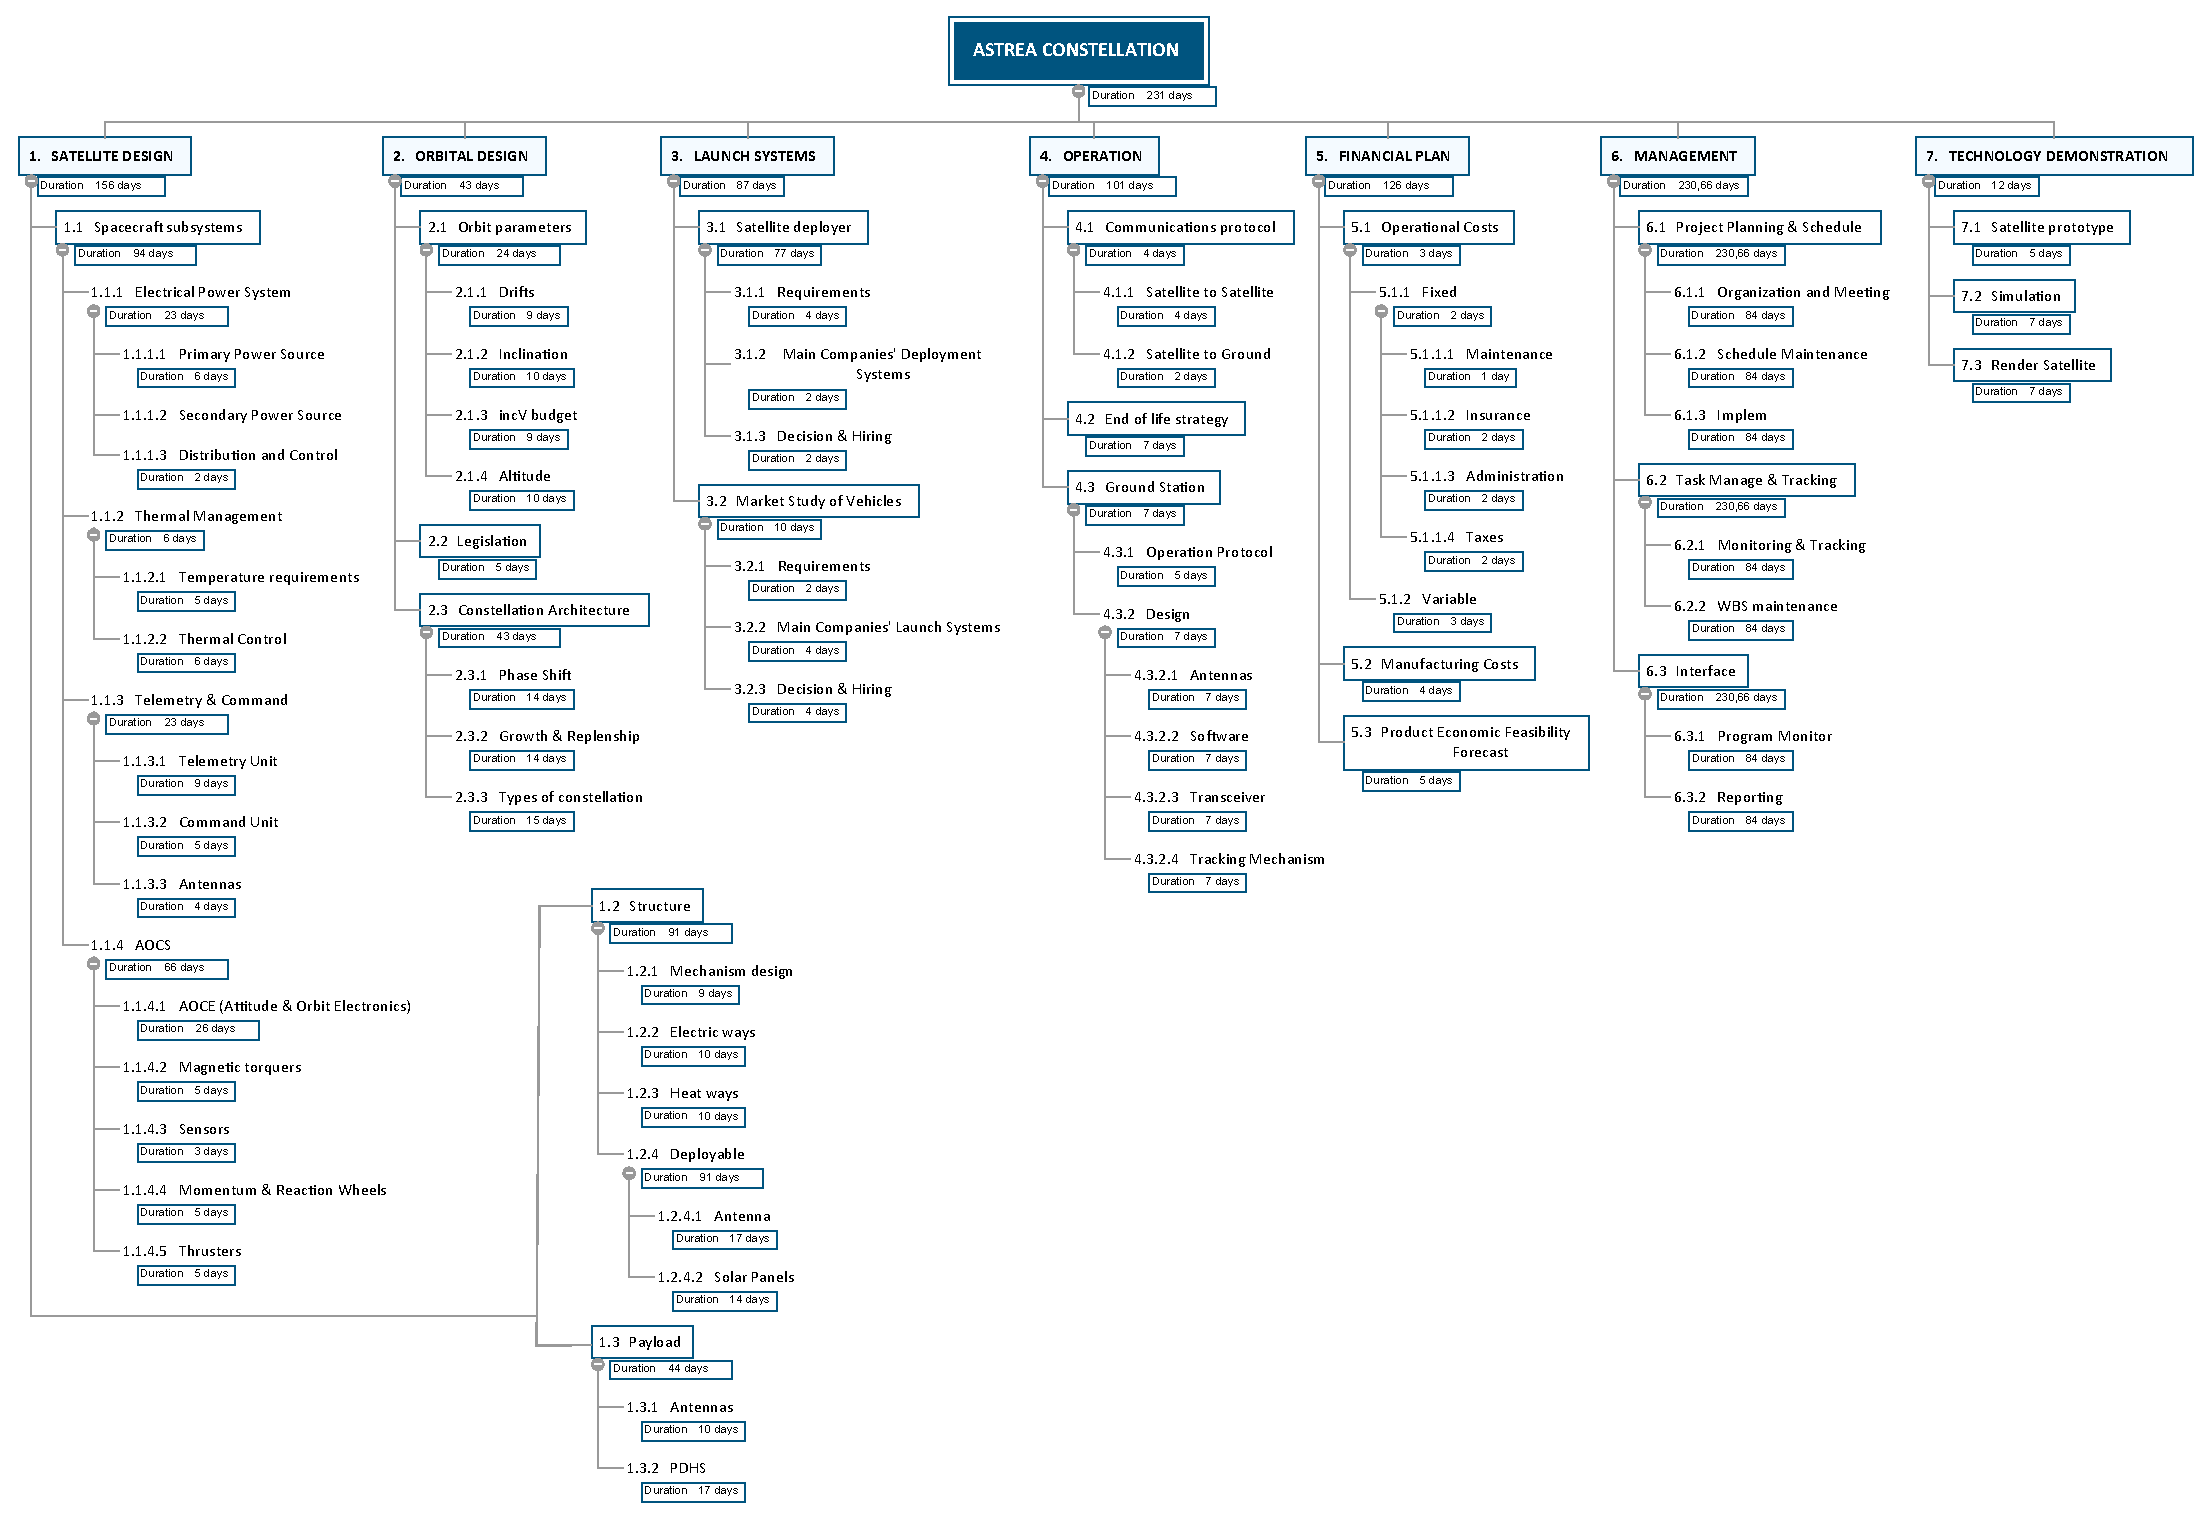
\includepdf[pages={1-}]{./external_pdf/wbs.pdf}

\subsection{Brief tasks description}


\subsection{Interdependency relationship among tasks}
\includepdf[pages={1-}]{./external_pdf/gantt.pdf}

%\subsection{Human resources and level of effort (hours) to develop each task}
%This is time for all good men to come to the aid of their party!
%
%\paragraph{Outline}
%The remainder of this article is organized as follows.
%Section~\ref{justification} gives account of previous work.
%Our new and exciting results are described in Section~\ref{justification}.
%Finally, Section~\ref{justification} gives the conclusions.


\section{Budget (initial estimation for engineering basic project)}
\includepdf[pages={1-}]{./external_pdf/budget.pdf}

\pagebreak
%\bibliographystyle{abbrv}
%\bibliography{simple}

\end{document}
